\documentclass[]{scrartcl}
\usepackage{graphicx}
\usepackage[dvipsnames]{xcolor}
\definecolor{mygray}{gray}{0.9}

% Title Page
\title{\textbf{Parallel computing - Exercise 3}}
\author{Michela Venturini}
\date{Spring 2019}

\begin{document}
\maketitle

\section{Compute \texttt{pi} by using MPI}
The aim of the exercice is to approximate the value of pi using the \textit{midpoint formula}. The code is implemented in the parallelized by using MPI and it is visible in the file \textit{ex3.c}. The implementation reduces the result in the last process with \texttt{rank=npes-1} and print the final output in the process with \texttt{rank=0}.

\section{Execution}
The code described is executed on Ulysses through a script (\textit{ex3.sh}) for 1,4,8,16,20, 32 and 40 threads and the time of execution is obtained by using \texttt{MPI\_Wtime()}.
The execution is performed by submitting a job on Ulysses through the command	\colorbox{mygray}{\texttt{qsub -l nodes=2:ppn=20}}\\\colorbox{mygray}{\texttt{ex3.sh}} that asks for two nodes.


\section{Results}
 The result of executions are stored in the file \textit{results.txt}. The Figure \ref{fig_1} shows the performance for the MPI case only; the Figure \ref{fig_2} shows a comparison between the OpenMP (using \texttt{atomic} directive) and the MPI implementations. In both cases the parameter n is set as \texttt{n=10e8}. The performance of \texttt{OpenMP} implementation are slightly better with respect to the other implementation until 16 threads, but both scale well. 
 
 \begin{figure}[h!]
 	\begin{centering}
 		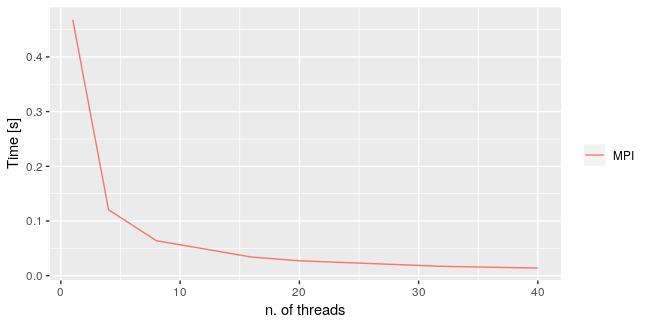
\includegraphics[scale=1]{mpi}
 		\caption{MPI implementation}
 		\label{fig_1}
 	\end{centering}
 \end{figure}

\begin{figure}[h!]
	\begin{centering}
		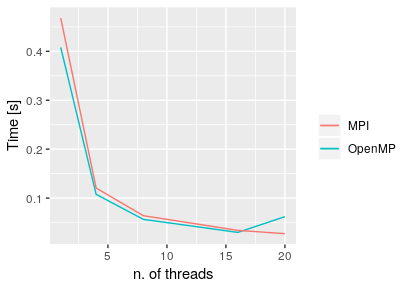
\includegraphics[scale=1]{plot_ok}
		\caption{Comparison between parallel implementations}
		\label{fig_2}
	\end{centering}
\end{figure}


\end{document}          
